\cotefile{10}
\scanpage{131}

b) Exemple d'un $\otimes$ foncteur exact fidèle, compatible avec $\deleted{\unsure{k\handwritten{\varphi}|k\handwritten{\psi}}}$ $1,\handwritten{\unsure{\varphi|\phi}},{}^{\handwritten{\unsure{\vee|\nu|v}}}$ (mais pas \deleted{avec} $\handwritten{\unsure{\psi|\varphi|\mu}}$ !), et qui n'est pas localement isomorphe au foncteur fibre donné. - On prend pour $G$ un groupe. On note alors que la donnée d'un système de $\deleted{W}\handwritten{L}_{g}$ et d'isomorphismes $(*)$ \deleted{avec $(**)$}, satisfaisant les diverses compatibilités, est équivalente à la donnée d'une extension de $G$ par $k^{\handwritten{*}}$. Le foncteur $\inserted{F'}$ est isomorphe \unsure{au|ay} foncteur $F$ sss cette extension splitte. L'ensemble des classes d'isomorphie de foncteurs fibres définis sur $k$ est ainsi en correspondance 1-1 avec $H^{2}(G,k^{\handwritten{*}})$. Or Même si $G$ est commutatif (par exemple le produit de deux groupes cycliques isomorphes d'ordre premier à \deleted{$k^{\handwritten{*}}$) et $k$} $\mathrm{car}.k$) et $k$ algébriquement clos, le $H^{2}$ peut être non nul; \deleted{\unsure{il ne se tue alors dans}} d'ailleurs un élément non nul de $H^{2}$ ne se tue dans aucune extension de $k$ (si $k$ alg. clos), d'après le principe de l'\unsure{extension|extensiion} finie.

Si cependant $G$ est commutatif, et si on se borne aux $F'$ compatibles avec $\handwritten{\psi}$ également, on trouve les extensions commutatives de $G$ par $k^{\handwritten{*}}$; si $k$ est algébriquement clos, donc $k^{\handwritten{*}}$ divisible, alors toute telle extension splitte, donc $F'$ est alors isomorphe à $F$ (en \unsure{confôrmité|conformité} avec la théorie galoisienne relative au cas où l'application diagonale de $U$ est commutative ...).

Ainsi, il peut y avoir des foncteurs fibres compatibles avec $\handwritten{\psi}$ donné, et d'autres qui ne le sont pas et qui par suite ne sont pas loc. isom. au premier. Cela montre donc \margin{\handwritten{\unsure{étudier} les contraintes de comm. \unsure{+|\&} \unsure{associon|assoc.} \unsure{aux graduations|des graduations} mod 2.}} \unsure{qu'on|qu'ôn} ne peut négliger la \deleted{condition de} contrainte de commutativité comme on aurait aimé pouvoir le faire. De plus, \margin{\figure{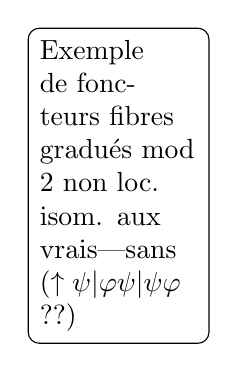
\begin{tikzpicture}
\node[text width=2cm,inner sep=4pt] (n) {\handwritten{Exemple de foncteurs fibres \unsure{gradués} mod 2 non loc. isom. aux \unsure{vrais|sans} $(\unsure{\uparrow\psi|\varphi\psi|\psi\varphi}$ ??)}};
\draw[rounded corners] (n.north west) -- (n.north east) -- (n.east) -- (n.south east) -- (n.south west) -- cycle;
\end{tikzpicture}}} cela suggère qu'en l'absence de contrainte de commutativité, la classification des foncteurs fibres se fait par des groupes du type de cohomologie de Brauer.

% archive sheet number: 130
\scanpage{132}

Dans cet exemple, on voit tout de suite qu\deleted{e}'il y a sur $C$ une \unsure{contrainte} de commutativité compatible avec les qutres données sss $U$ est commutatif c'est à dire $G$ est commutatif, et que lesdites contraintes correspondent \inserted{alors} aux fonctions $: G\unsure{\times|x}G\handwritten{\unsure{\rightarrow|-}} k^{\handwritten{*}}$ qui sont bilinéaires et antisymétriques. Dans le cas où le $H^{2}(G,k^{\handwritten{\unsure{*|'}}})$ est \inserted{géométriquement} nul (par exemple $G$ cyclique \deleted{et $k$ algébriquement clos}) on voit donc que pour tout choix non nul de $\handwritten{\sigma}$, on a une contrainte de commutativité pour laquelle il n'y a aucun foncteur fibre compatible avec ladite contrainte (et les \unsure{autres)} sur aucune extension de $k$. On peut songer à s'en tirer en trouvant au moins des foncteurs fibres gradués compatibles à toutes les contraintes mais on voit déjà que c'est impossible si $k$ de car.deux (où il n'y a pas de différence entre l'existence de l'un et l'autre type de foncteur fibre, gradué ou non); et sans doute l'analyse doit montrer que l'on a un même résultat négatif en toute caractéristique. Noter cependant dans ces exemples on pouvait au moins, en modifiant la contrainte de commutativité donnée, en trouver une qui admette un foncteur fibre compatible à ladite contrainte. Il y aurait donc lieu de donner un exemple d'une $\otimes$-catégorie définissable par une bialgèbre\deleted{\unsure{s}}, admettant une contrainte de commutativité (compatible au reste) mais aucune cont\deleted{\unsure{m|n}}rainte de commutativité pour laquelle on puisse \unsure{trouver|frouver} un foncteur fibre (gradué au besoin):sur aucune extension du corps donné.

\handwritten{Avec les notations du n° 11, il faudra \unsure{donc} $\Delta_{U}$ \inserted{i.e. $A$} non commutatif\inserted{\unsure{vu!|u.!}}, et $U$ non commutatif (sinon l'existence de $\sigma$ impliquerait la commutativité de $\Delta$).}
% archive sheet number: 131
\scanpage{133}

c) Soit $X$ un schéma \deleted{complet}\inserted{propre} sur un corps $k$, supposons $H^{\unsure{0|o}}(X,\underline{O}_{X})=k$. La catégorie $\inserted{C}$ des faisceaux cohérents sur $X$ est une catégorie avec $\otimes,\handwritten{\unsure{\varphi|\phi}},\handwritten{\unsure{\psi|\varphi|\mu}},$ \deleted{Hom} $1$, \uline{Hom} internes, \inserted{\handwritten{$\mathrm{Hom}(X,Y)$ de dim. finie sur $k$,}} mais l'homomorphisme $\unsure{X|X^{\handwritten{\vee}}}\otimes Y\handwritten{\simeq}\underline{\mathrm{Hom}}(X,Y)$ \uline{n'est pas un isomorphisme}\inserted{(axiome de rigidité)}. C'est pour cela qu'il n'y a pas lieu de s'attendre à une vraie théorie de Galois de $\deleted{\unsure{X}}C$. Il y a des foncteurs fibres associés aux divers points de $X$ (pas nécessairement fermés), à $x$ correspond un foncteur fibre défini sur $k(x)$; sans doute\deleted{\unsure{s|x}} il n'y en a pas d'autres à isomorphisme près (à vérifier). Ils\deleted{\unsure{s|x}} ont toutes les compatibilités, mais \uline{ils ne sont pas exacts}, \deleted{Pour y rém} \uline{ni fidèles}. Pour remédier au défaut d'exactitude, sans que $C$ cesse d'être abélienne (sinon on prendrait les Modules loc. libres seulement !), on peut se fixer un ouvert $U\quad X$ et définir $C$ en prenant des Faisceaux cohérents qui, sur $U$, sont munis d'une stratification relativement à $k$: tout point $x\handwritten{\in}\unsure{\mathbb{U}|U}$ fournit un foncteur fibre exact. Cependant, si $U\handwritten{\not}=X$, ce foncteur ne sera pas fidèle. Bien sûr, si $U=X$, l'áxiome de rigidité est satisfait, et on sait qu'on a une théorie de Galois. Il doit résulter de cette dernière que $C$ n'a pas de foncteur fibre (compatible avec toutes les données) sur une extension de $k$ (car autrement l'axiome de rigidité serait satisfait).

\uline{A prouver:} Soit $C$ une catégorie \inserted{abélienne} avec $\otimes_{\deleted{\unsure{k|x}}}$ biadditif, $\handwritten{\varphi},\handwritten{\psi},1,{}^{\handwritten{\unsure{\vee|\nu|v}}}$ et rigidité. Alors a) $\inserted{k=}\mathrm{End}(\unsure{\mathbb{1}|1})$ est un anneau absolument plat, donc un composé fini de \deleted{\unsure{orops|orps|corps}} corps s'il est noethérien. b) Les $\mathrm{Hom}(\unsure{\mathbb{X}|X},Y)$ sont des modules de présentation finie \inserted{i.e. cohérents} sur $k$ (NB les modules de présentation finie sur $k$ forment une catégorie abélienne, en fait $k$ est un anneau ``cohérent''). c) \deleted{Toute sous-catégorie de $C$ stable par tout et à \unsure{engend}} $C$ est limite inductive de sous-catégories (en général pas pleines) stables par tout, y compris noyaux, conoyaux, ${}^{\handwritten{\vee}}$, $\otimes$, et correspondants à des anneaux $k_{i}$ qui sont des \deleted{sommes} composés de corps. d) Le cas d'un composé de corps se ramène à celui d'un corps.
% archive sheet number: 132
\scanpage{134}

1\deleted{2}\handwritten{3}) Variante utile du tapis de n° 6. Soit $C$ une catégorie, et $\deleted{\unsure{F:C\;\mathrm{Mo}|F:C\;\mathrm{Mod}}}$
\[
F:C\handwritten{\longrightarrow}\mathrm{Modf}(k)
\]
un foncteur, où $\deleted{\unsure{j|t}}k$ est un corps. On ne suppose pas $C$ additive, ni $F$ fidèle. On définit alors l'anneau profini $U=\mathrm{End}_{k}(F)$, la coalgèbre duale $A$, et on trouve une factorisation canonique de $F$ à travers $\mathrm{Modf}(U/k)=\mathrm{Comodf}(A/k)$. Supposons donné dans $C$ un bifoncteur $\otimes$, \deleted{alors}\inserted{\handwritten{et}} un isomorphisme de bifoncteurs $F(X\otimes Y)\handwritten{\simeq}F(X)\otimes F(Y)$, alors on trouve une application diagonale sur $U$ i.e. une loi de composition \deleted{\unsure{comp|comp.} avec \unsure{appli}} sur $A$: en effet, on constate que l'anneau des endomorphismes du bifoncteur du premier membre est $U\otimes_{k}U$, et $U$ s\deleted{e}'envoie dedans grâce à l'isomorphisme donné $F(X\otimes Y)\handwritten{\simeq}F(X)\otimes F(Y)$. Si on se donne pour $\otimes$ des données d'unité, d'associativité ou de commutativité, la compatibilité de ces données avec $c$ s'exprime alors comme il est dit dans n° 6\inserted{\handwritten{en termes de $\Delta$}}, et il y a lieu de donner des variantes graduées (si possible plus générale\handwritten{s} et astucieuse\handwritten{s} qu'au n° 8\handwritten{)}. En fait, les résultats spécifiques au n°6 seraient \unsure{plûtôt|plutôt}, dans le cas d'un foncteur \unsure{fi\`{d}èle|fièèle|fidèle} (et additif \deleted{\unsure{de caté}} exact de catégories abéliennes ? à voir de quoi exactement on a besoin), des réciproques aux constructions précédentes, i.e. comment déduire d'une application diagonale sur $U$ un\deleted{\unsure{e|x}} foncteur $\otimes$ sur $C$, do\deleted{j}nt les \unsure{pr\deleted{i}opriétés|pròpriétés|propriétés} vont réfléter celles de cette dernière.

Exemple intéressant: les opérations cohomologiques sur $\underline{F}_{p}$. Il mérite quelques explications: sauf le morceau engendré par les $\handwritten{\pi}_{i}$ \deleted{(NB $\unsure{i|1}$} les degrés dans $U$ sont $\handwritten{>}$ $0$, et $\overset{\handwritten{\sim}}{U}\inserted{\handwritten{=k+U^{+}}}$ est le complété c\unsure{aa|an|na}onique d'un anneau gradué à application diagonale anticommutative, donc $\overset{\handwritten{\sim}}{A}$ est un anneau analogue. Dire comment on récupère $U,A$ à partir de $\overset{\handwritten{\sim}}{U}$, $\overset{\handwritten{\unsure{\sim}}}{\overset{\handwritten{\sim}}{A}}$.
% archive sheet number: 133
\scanpage{135}

Théorème de \handwritten{- - - - - -} (rapporté par Husemöller).

Soit $A$ une bialgèbre sur le corps $k$, $A$ associative et unitaire pour ses deux structures, ``cocomplète'' pour sa filtration canonique de comodule (duale de la filtration par les puissances de l'idéal d'augmentation du dual; de façon précise, écrivant $\overset{n}{\otimes}A=\overset{n}{\otimes}A^{\handwritten{+}}+$ fou\uline{r}bis, d'où via la m.ème itéré\deleted{\unsure{e|s}} du morphisme diagonal, une application $A\handwritten{\longrightarrow}\overset{n}{\otimes}I^{\handwritten{+}}$, dont le noyau\inserted{\handwritten{\unsure{intersect°|intersect.} avec $A^{+}$}} est $\mathrm{Filt}_{m}(A)$).\margin{\handwritten{cela entraîne qu'il y a un \unsure{antipodisme} ?}} (NB l'hypothèse cocomplète est satisfaite pour une coalgèbre \inserted{avec unité} à degrés $\handwritten{\geq}$ $0$ réduite à $k$ en degré\deleted{s} $0$, associative et unitaire, - parait-il !). Soit $M$ un $A$-module, muni d'un homomorphisme diagonal \inserted{sur $k$} unitaire (peut-être pas associatif), $M\handwritten{\longrightarrow}M\otimes_{k}M$, qui soit $A$-linéaire\unsure{,|.}\margin{\figure{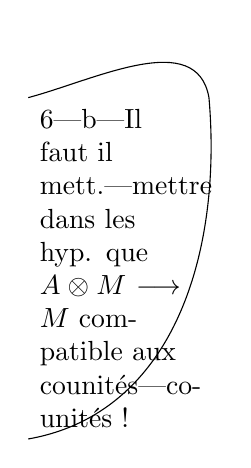
\begin{tikzpicture}
\node[text width=2cm,inner sep=4pt] (n) {\handwritten{\unsure{6|b|Il} faut il \unsure{mett.|mettre} dans les hyp. que $A\otimes M\longrightarrow M$ compatible aux \unsure{counités|co-unités} !}};
\draw (n.north west) to[out=15,in=100] (n.north east) to[out=-85,in=10] (n.south west);
\end{tikzpicture}}}\inserted{\handwritten{(pour la structure de $A$-module sur $M\otimes M$ provenant de $A\longrightarrow A\otimes A$; il revient au même de dire que $A\otimes M\longrightarrow M$ comp. avec application diagonale)}} Supposons de plus donné une ``unité'' i.e. un homomorphisme $k\handwritten{\longrightarrow}M$ qui soit un homomorphisme de coalgèbres unitaires, i.e. $\underset{M}{\mathrm{L}}$'image $\inserted{e_{M}}$ de $1$ satisfait $\handwritten{\unsure{\epsilon|\varepsilon}}_{M}(e_{M})=1$, $\handwritten{\Delta}_{M}(e_{M})=e_{M}\otimes e_{M}$. Supposons également $M$ cocomplète, et que\deleted{on} l'application $u\handwritten{\mapsto}u.e$ de $A$ dans $M$ soit injective. Alors $M$ est un $A$-module libre, \inserted{\handwritten{ayant une base dont fait partie $e$;}} de façon plus précise, posant $\overset{\handwritten{-}}{M}=M\otimes_{A}k$, il existe un isomorphisme (non canonique ...) de $A$-modules $M\handwritten{\overset{\sim}{\unsure{\longleftarrow|\longleftrightarrow}}}A\otimes_{k}\overset{\handwritten{-}}{M}$\handwritten{, tel que le diagramme}
\margin{\handwritten{?}}
\handwritten{\diagram{\begin{tikzcd}[ampersand replacement=\&,column sep=small,row sep=small]
M \arrow[dr] \& \& \unsure{A|\mathcal{A}}\otimes_{k}\overline{M} \arrow[ll,"\sim"'] \arrow[dl] \\
\& \overline{M} \&
\end{tikzcd}}}
\handwritten{\unsure{commute|commuta}, et que ...}

Exemple \handwritten{1}. Supposons l'application diagonale de $A$ commutative. Alors $A$ peut être considéré comme l'hyperalgèbre d'un groupe formel connexe $\inserted{G}$ sur $k$. Si $\handwritten{\Delta}_{M}$ est associatif et commutatif, $M$ aussi est formé des distributions à l'origine d'une variété formelle connexe $\inserted{V}$ sur $k$, et le fait que $A$ opère sur $M$ de façon que l'application diagonale soit $A$-linéaire signifie que $G$ opère sur $V$. On voit donc que si $u\handwritten{\unsure{\vdash|\mapsto}}\unsure{\mathbb{U}|\mathbb{u}|U|u}.e$ \inserted{de $A$ dans $M$} est injectif, i.e. si $g\handwritten{\mapsto}g.a$ ($a$ le `centre' de $V$) de $G$ dans $V$ est un monomorphisme, alors $M$ est libre sur $A$. En fait, on trouvera que $G$ opère librement sur $V$ i.e.
% archive sheet number: 134
\scanpage{136}
que $G\unsure{\times|x}V\handwritten{\longrightarrow}V\times V$ est un monomorphisme (c'est le lemme de Nakayama), et on sait bien alors (SGA 3 $\mathrm{VII}_{\mathrm{B}}$ ...) que \deleted{$V$ est un} l'on a un joli quotient $W=V/G$, avec $\deleted{W\quad V}$ $V\handwritten{\longrightarrow}W$ plat et en fait la projection structurale d'un $G_{W}$-torseur. Bien sûr la coalgèbre $\overset{\handwritten{-}}{M}$ n'est autre que celle qui définit le quotient $W$ précédent. En général, il n'est pas question de prouver que $V\handwritten{\simeq}W\times G$ comme variété formelle à opérateurs (i.e. que le torseur précédent est trivial), i.e. de trouver une\deleted{isomorphisme} section de $V$ sur $W$, i.e. un relèvement de comodules $\overset{\handwritten{-}}{M}\handwritten{\longrightarrow}M$; on peut seulement dire que tout relèvement en tant que $k$-vectoriels définira un isomorphisme $A\otimes_{k}\overset{\handwritten{-}}{M}\handwritten{\simeq}M$ de $A$-modules. Cependant, si $G$ est formellement lisse i.e. le dual de $A$ une algèbre de péries formelles (éventuellement à un nb infini de générateurs) alors on aura splittage parfait; ce sera la cas en particulier en car. nulle.

\uline{Exemple} 2. Supposons $A$ commutative pour sa loi d'algèbre. Donc $A$ est l'algèbre affine d'un schéma en monoïdes \inserted{affine} $G$. L'hypothèse sur la filtration coc\deleted{\unsure{c}}omplète est assez étrange ici, elle s'énonce en disant que pour toute $f\handwritten{\in}A$ (fonction sur $G$) \deleted{nulle en $e$}, il existe un entier $n\inserted{\handwritten{\geq\unsure{2|1}}}$ tel que la fonction en $n$\deleted{\unsure{s|x}} variables $f(g_{1}g_{2}\ldots g_{n})$ soit \deleted{identiquement nulle}\inserted{somme de fonctions} à $n-1$ parmi les \unsure{varaables|variables}.\margin{\figure{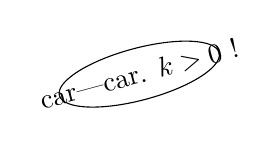
\begin{tikzpicture}[rotate=15,transform shape]
\node[inner sep=3pt] (n) {\handwritten{\unsure{car|car.} $k>0$ !}};
\draw (n.center) ellipse [x radius=1.05cm,y radius=0.33cm];
\end{tikzpicture}}} Si $G$ est de type fini sur $k$\inserted{\handwritten{de car $p>0$}}, je pense que \deleted{dès qu'on y remplace une des variables par $1$, mais alors, faisant tous} cela doit entraîner que \deleted{l'unité de} $G$ est \deleted{point isolé, donc,\deleted{si $G$ est un} \deleted{les arguments \unsure{suffirien|suffirion|suffiront}} comme $G$ est un groupe, que \deleted{groupe, que} $G$ est fini sur $k$. \deleted{Dans dans le cas général, que $G$ est profini sur $k$.} Si $G$ est commutatif (i.e. $\handwritten{\Delta}_{A}$ commutatif), alors le dual de Cartier de $A$ doit être purement infinitésimal, i.e. $G$ doit être unipotent (et réciproquement). On peut conjecturer que \deleted{la con} la condition en question, pour $G$ de type fini pas néc. comm., équivaut à $G$ fini unipotent.}\margin{\handwritten{?}}\inserted{\handwritten{unipotent}} donc si on ne suppose plus nom plus $G$ de type fini, que $G$ est \deleted{\unsure{profini et|profini}} prounipotent.

% archive sheet number: 135
\scanpage{137}

\uline{Corollaire} Supposons que l'homomorphisme $M\handwritten{\longrightarrow}M\otimes_{k}M$ induise un homomorphisme $M\otimes_{(A,\handwritten{\Delta}_{A})}(A\otimes_{k}A)\quad M\otimes_{k}M\deleted{\unsure{,|x}}$ \deleted{donc par réduction} qui soit un \uline{isomorphisme} Alors l'homomorphisme $u\handwritten{\mapsto}u.e$ de $A$ dans $M$ est un isomorphisme pour toutes les structures.

Il suffit de prouver que le rang $\inserted{n}$ de $M$ sur $A$ est $1$. Or ce rang de $M\otimes_{k}M$ sur $A\otimes_{k}A$ est $n^{2}$, et on aura $n=n^{2}$, i.e. $n(n-1)=0$ d'où, comme $n\handwritten{\not}=0$, $n=1$. Ceci ne marche que si on sait que le rang est \unsure{fini|mini}. Mais on peut dire aussi que l'application diagonale pour $\overset{\handwritten{-}}{M}$, déduite de celle de $M$ par passage au quotient (NB $\overset{\handwritten{-}}{M}\otimes\overset{\handwritten{-}}{M}=(M\otimes_{k}M)\otimes_{(A\otimes_{k}A)}k$) est \uline{surjective}, donc bijective puisqu'elle est unitaire, donc tout élément de $\overset{\handwritten{-}}{M}\otimes\overset{\handwritten{-}}{M}$ est de la forme $\overset{\handwritten{-}}{e}\otimes x$, ce qui n'est possible que si $\overset{\handwritten{-}}{e}$ engendre $\overset{\handwritten{-}}{M}$.

Ceci montre que la conjecture de locale trivialité \unsure{soulevée|sonlevée} dans mes notes sur les $\otimes$-catégories marche si la bialgèbre $A$ \unsure{envisagëe|envisagée|enfisagëe|enfisagée} est finie sur $k$\inserted{et sa duale est cocomplète,} \uline{pourvu que} l\deleted{a}'algèbre $B$ admette un homomorphisme d'algèbres dans $k$ (ou une extension de $k$), i.e. pourvu que $B$ ne soit pas identique à son idéal des commutateurs.
% archive sheet number: 136
